\documentclass{article}
\usepackage[utf8]{inputenc}
\usepackage{tikz}
\usepackage{siunitx}
\usepackage{graphics}
\usepackage[american,siunitx]{circuitikz}
\usepackage{amsmath}
\usepackage{svg}
\usepackage{booktabs}
\usepackage{float}
\usepackage{xparse, xfp}
\usepackage{graphicx} 
\usepackage{steinmetz}
\usepackage{hyperref}
\usepackage{scalerel}
\usetikzlibrary{angles,quotes}
\renewcommand{\thesubsubsection}{\thesubsection.\alph{subsubsection}}
\newcommand{\equal}{=}

\title{ECE2101L\\Electrical Circuit Analysis II Laboratory\\\,\\Lab 9\\Real, reactive, complex power and power factor\\\,\\Prelab\\}
\author{Choi Tim Antony Yung}
%\author{Choi Tim Antony Yung\\\,\\Willis Nguyen\\Phineas Cozmiuc}

\begin{document}

\clearpage\maketitle
\thispagestyle{empty}
\newpage
\setcounter{page}{1}

\section{Power calculation}
Given $Z=35\phase{-27^{\circ}}\Omega$ and $I=52\phase{43^{\circ}}$A:

\subsection{Real, reactive, apparent, and complex power}
\subsubsection{Complex Power}
$$S=VI^*=IZI^*=I_{rms}^2Z = \frac{52^2}{2}35\phase{-27^{\circ}}$$
$$S=47320\phase{-27^{\circ}}=42162-21483j\text{\,VA}$$
\subsubsection{Real Power}
$$P=42162\text{\,W}$$
\subsubsection{Reactive Power}
$$Q=-21483\text{\,VAR}$$
\subsubsection{Apparent Power}
$$|S|=47320\text{\,VA}$$

\subsection{Power factor}
$$PF=cos(\theta_v-\theta_i)=cos(arg(Z))=cos(-27^{\circ})=0.8910$$
As $Q<0$, the power factor is leading.

\subsection{Load power triangle and load impedance triangle}
\begin{figure}[H]   
    \centering
    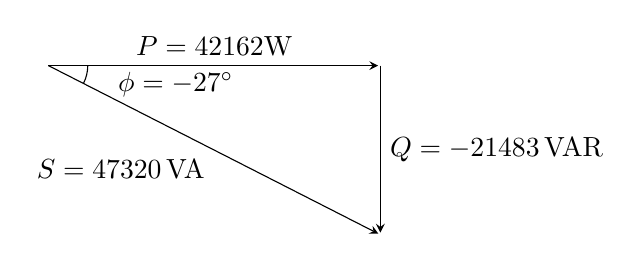
\begin{tikzpicture}[scale=1]
        \path[-stealth,shorten >=0.8pt] (0cm,0cm) coordinate (A) 
        (4.2162cm,-2.1483cm) coordinate  (B)
        (4.2162cm,0cm) coordinate  (C)
        (A) edge["$S = 47320 \text{\,VA}$"'] (B) 
        (C) edge["$Q = -21483\text{\,VAR}$"] (B) 
        (A) edge["$P = 42162 \si{\watt}$"] (C);
        \path let \p1=($(B)-(A)$) in
        pic["$\alpha$",draw,angle eccentricity=1.1,"$\pgfmathparse{atan2(\y1,\x1)}
        \phi=\pgfmathprintnumber{\pgfmathresult}^\circ$"
        {anchor=west,xshift=1.5ex,yshift=-.75ex}] {angle=B--A--C};
    \end{tikzpicture}
    \caption{Load Power Triangle}
\end{figure}
\begin{figure}[H]   
    \centering
    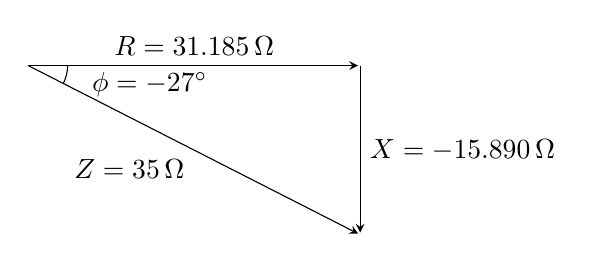
\begin{tikzpicture}[scale=1]
        \path[-stealth,shorten >=0.8pt] (0cm,0cm) coordinate (A) 
        (4.2162cm,-2.1483cm) coordinate  (B)
        (4.2162cm,0cm) coordinate  (C)
        (A) edge["$Z =  \SI{35}{\ohm}$"'] (B) 
        (C) edge["$X = \SI{-15.890}{\ohm}$"] (B) 
        (A) edge["$R =  \SI{31.185}{\ohm}$"] (C);
        \path let \p1=($(B)-(A)$) in
        pic["$\alpha$",draw,angle eccentricity=1.1,"$\pgfmathparse{atan2(\y1,\x1)}
        \phi=\pgfmathprintnumber{\pgfmathresult}^\circ$"
        {anchor=west,xshift=1ex,yshift=-.75ex}] {angle=B--A--C};
    \end{tikzpicture}
    \caption{Load Impedance Triangle}
\end{figure}

\section{The above calculation was reproduced in MATLAB}
\begin{figure}[H]
    \centering
        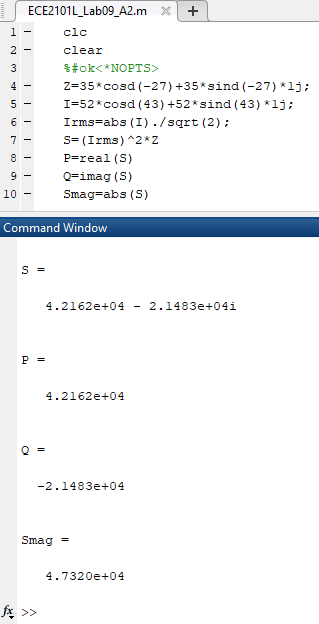
\includegraphics[scale=0.8]{ECE2101L_Lab09_A2.png}
\end{figure}

\end{document}